\documentclass{article}
\title{AG1 - Cvičení I}
\author{Tommy Chu}
\date{}

\usepackage[czech]{babel}
\usepackage[utf8]{inputenc}
\usepackage[T1]{fontenc}
\usepackage{graphicx}
\usepackage{amsmath}
\usepackage{amsthm}
\usepackage{amssymb}
\usepackage{subfiles}
\usepackage{hyperref}
\usepackage{geometry}
\usepackage{mathtools}
\usepackage{algpseudocode}
\usepackage{algorithm}
\usepackage{physics}
\usepackage{dsfont}
\usepackage{bm}
\usepackage{bbm}
\usepackage{float}
\usepackage{enumitem}
\usepackage{graphicx}
\usepackage{multirow}
\usepackage{tikz}
\usepackage{tikz-cd}
\usepackage{pgfplots}
\usepackage{lmodern}
\usepackage{import}
\usepackage{microtype}
\usepackage{fancyhdr}
\usepackage{parskip}

\usepackage{mystyle}

\begin{document}
\maketitle

\section*{Zadání 1}

Ukažte, že pro každé $n \ge 2$ existuje graf na vrcholech $v_1, \dots, v_n$ takový, že existuje nanejvýš jedna dvojice indexů $i \ne j$ taková, že $\deg v_i = \deg v_j$. Jinými slovy všechny vrcholy mají různé stupně až na dva.

\subsection*{Řešení}

Graf na $n$ vrcholech splňující podmínku v zadání neobsahuje dvojici vrcholů stupně 0. Pokud by takové vrcholy existovaly, musely by zbylé vrcholy být minimálně stupně $1, 2, \dots, (n-2)$. Nicméně vrcholy v tomto grafu mohou být nejvýše stupně $(n-3)$, protože z celkových $n$ vrcholů by 2 vrcholy byly izolované a vrchol nemůže sousedit sám se sebou.

Analogicky lze ukázat, že neexistuje graf, který by měl dvojici vrcholů stupně $(n-1)$ -- nevycházel by vrchol se stupněm 0 nebo 1.

Pro jednoduchost se budeme v důkazu strikně držet pouze grafů bez izolovaných vrcholů.

Definujme výrok $V(n)$ následovně:
\begin{align*}
    V(n) \Longleftrightarrow \;
     & \text{existuje graf na vrcholech $v_1, . . . , v_n$ takový, že existuje}       \\
     & \text{\textbf{právě jedna} dvojice indexů $i \ne j$ kde $\deg v_i = \deg v_j$}
\end{align*}

Platnost $V(n)$ pro všechna $n \ge 2$ dokážeme matematickou indukcí.

\textbf{Základní krok:} Dokážeme tvrzení pro $n = 2$ a $n = 3$. Grafy splňující $V(2)$ a $V(3)$ jsou například:

\begin{center}
    \begin{tikzpicture}[node distance={15mm}, main/.style = {draw, circle}]
        \node[main] (1) {$v_1$};
        \node[main] (2) [right of = 1] {$v_2$};
        \draw (1) -- (2);
    \end{tikzpicture}
    \qquad
    \begin{tikzpicture}[node distance={15mm}, main/.style = {draw, circle}]
        \node[main] (1) {$v_1$};
        \node[main] (2) [right of = 1] {$v_2$};
        \node[main] (3) [right of = 2] {$v_3$};
        \draw (1) -- (2);
        \draw (2) -- (3);
    \end{tikzpicture}
\end{center}

\textbf{Indukční krok:} Ukážeme, že platí $V(n) \Rightarrow V(n+1)$ pro všechna $n \ge 3$.

Předpoklad $V(n)$: Existuje graf $G=(V, E)$ na $n$ vrcholech, které mají různé stupně až na dva. Vzhledem k tomu, že neuvažujeme izolované vrcholy, tyto vrcholy mají nutně stupně $1, \dots, k, k, \dots, (n-1)$, kde jsou právě dva vrcholy stupně $k \in \{ 1, 2, \dots, (n-2) \}$. To vyplývá z toho, že stupně vrcholů jsou menší než $n$. A v souladu s úvodní poznámkou navíc musí platit $k < (n-1)$.

Vytvoříme graf $H$ rozšířením grafu $G$ o nový vrchol $u$ následujícím způsobem:
\begin{align*}
    H = (
    V \cup \{ u \}, E
     & \cup\{ \{u, v\} \mid v \in V \colon \deg_G v > k \}                      \\
     & \cup \{ \{u, v\} \mid \text{$v$ je jeden konkrétní vrchol stupně $k$} \}
    )
\end{align*}
Ukážeme, že graf $H$ dokazuje $V(n+1)$.

Všechny vrcholy stupně vyšší než $k$ a jeden z dvojice vrcholů stupně $k$ byly spojené s novým vrcholem $u$. Stupně vrcholů $V(H) \setminus \{u\}$ se od stupní vrcholů z původního grafu $G$ liší následovně:
\begin{align*}
    V(G) \colon \quad
     & 1, \dots, k, k, \dots, (n-1)                           \\
    V(H) \setminus \{u\} \colon \quad
     & 1, \dots, k, (k+1), \dots, n \quad = \quad 1, \dots, n
\end{align*}

Přidáním hran se zvedly stupně vrcholů s víc než $k$ sousedy o jedna. Tím se uvolnil stupeň $(k+1)$, který zabral jeden z vrcholů původně stupně $k$. Stupně vrcholů $V(H) \setminus \{u\}$ jsou proto rozdílné a jejich stupně jsou: $1, \dots, n$.

Stupeň přidaného vrcholu $u$ je
\begin{align*}
    \deg_H u & = |\{ \{u, v\} \mid v \in V \colon \deg_G v > k \}| + 1 \\
             & = |\{ v \in V \mid \deg_G v > k \}| + 1                 \\
             & = ((n - 1) - k) + 1                                     \\
             & = n - k \in \{ 1, \dots, (n-1) \}
\end{align*}

Existují tedy dva vrcholy stupně $(n-k)$.
Graf $H$ je na $(n+1)$ vrcholech a všechny jeho vrcholy mají různé stupně až na dva. Potvrdili jsme, že pokud platí $V(n)$ (existuje $G$), pak platí $V(n+1)$ (lze sestrojit $H$).

\textbf{Závěr:}
Podle slabého principu matematické indukce platí $V(n)$ pro $n = 2$ a $n \ge 3$.

Tvrzení $\forall n \ge 2 \colon V(n)$ je omezené na právě jeden pár vrcholů stejného stupně místo nanejvýše jednoho páru. Je proto postačující podmínkou pro větu v zadání.
\qed

\newpage
\section*{Zadání 2}

V hospodě se porvalo všech $2n+1$ návštěvníků. Každý dal ránu přesně $n$ různým kolegům. Dokažte, že existuje návštěvník hospody, který inkasoval ránu od někoho, komu on sám ránu nedal.

\subsection*{Řešení}

Nešťastný návštěvník je ten, který inkasoval ránu od někoho, komu on sám ránu nedal. Pokud nás nezajímá, zda nešťastný návštěvník existuje či ne, potom rvačka může vždy nastat -- např. následujícím způsobem: $2n + 1$ návštěvníků se postaví do kruhu a každý navštěvník dá ránu $n$ kolegům, které má bezprostředně po své pravé straně.

Pokusíme se nalézt situace, kdy nešťastný návštěvník neexistuje: Pokaždé když nějaký návštěvník dá někomu ránu, schytá to od toho samého ihned nazpět. Jinými slovy hledáme $n$-regulární graf na $2n+1$ vrcholech, kde každá hrana v grafu reprezentuje vzájemnou výměnu ran.
Pokud najdeme takový graf, vyvrátíme existenci nešťastného návštěvníka. Naopak, pokud ukážeme, že takový graf nelze sestrojit, dokážeme, že ve všech takových rvačkách nešťastný návštěvník jistě existuje.

\textbf{Liché $n$:} Graf nelze sestrojit. Neexistuje rvačka tvořena čistě ze vzájemných ran. Ve všech rvačkách je nešťastný návštěvník.
Kdyby takový graf $G = (V, E)$ existoval, byl by součet stupňů vrcholů lichý, což by nevyhovovalo principu sudosti:
\begin{align*}
    \sum_{v \in V} \deg v & = \sum_{v \in V} n = |V| \cdot n = (2n + 1) \cdot n \quad \leftarrow \text{součin dvou lichých čísel}
\end{align*}

\textbf{Sudé $n$:} Graf lze sestrojit. Existuje rvačka tvořená pouze vzájemnými ranami bez nešťastného návštěvníka.
Pro sudá $n$ můžeme tvrzení v zadání vyvrátit například následujícími protipříklady pro $n=2, 4, 6$:

\begin{center}
    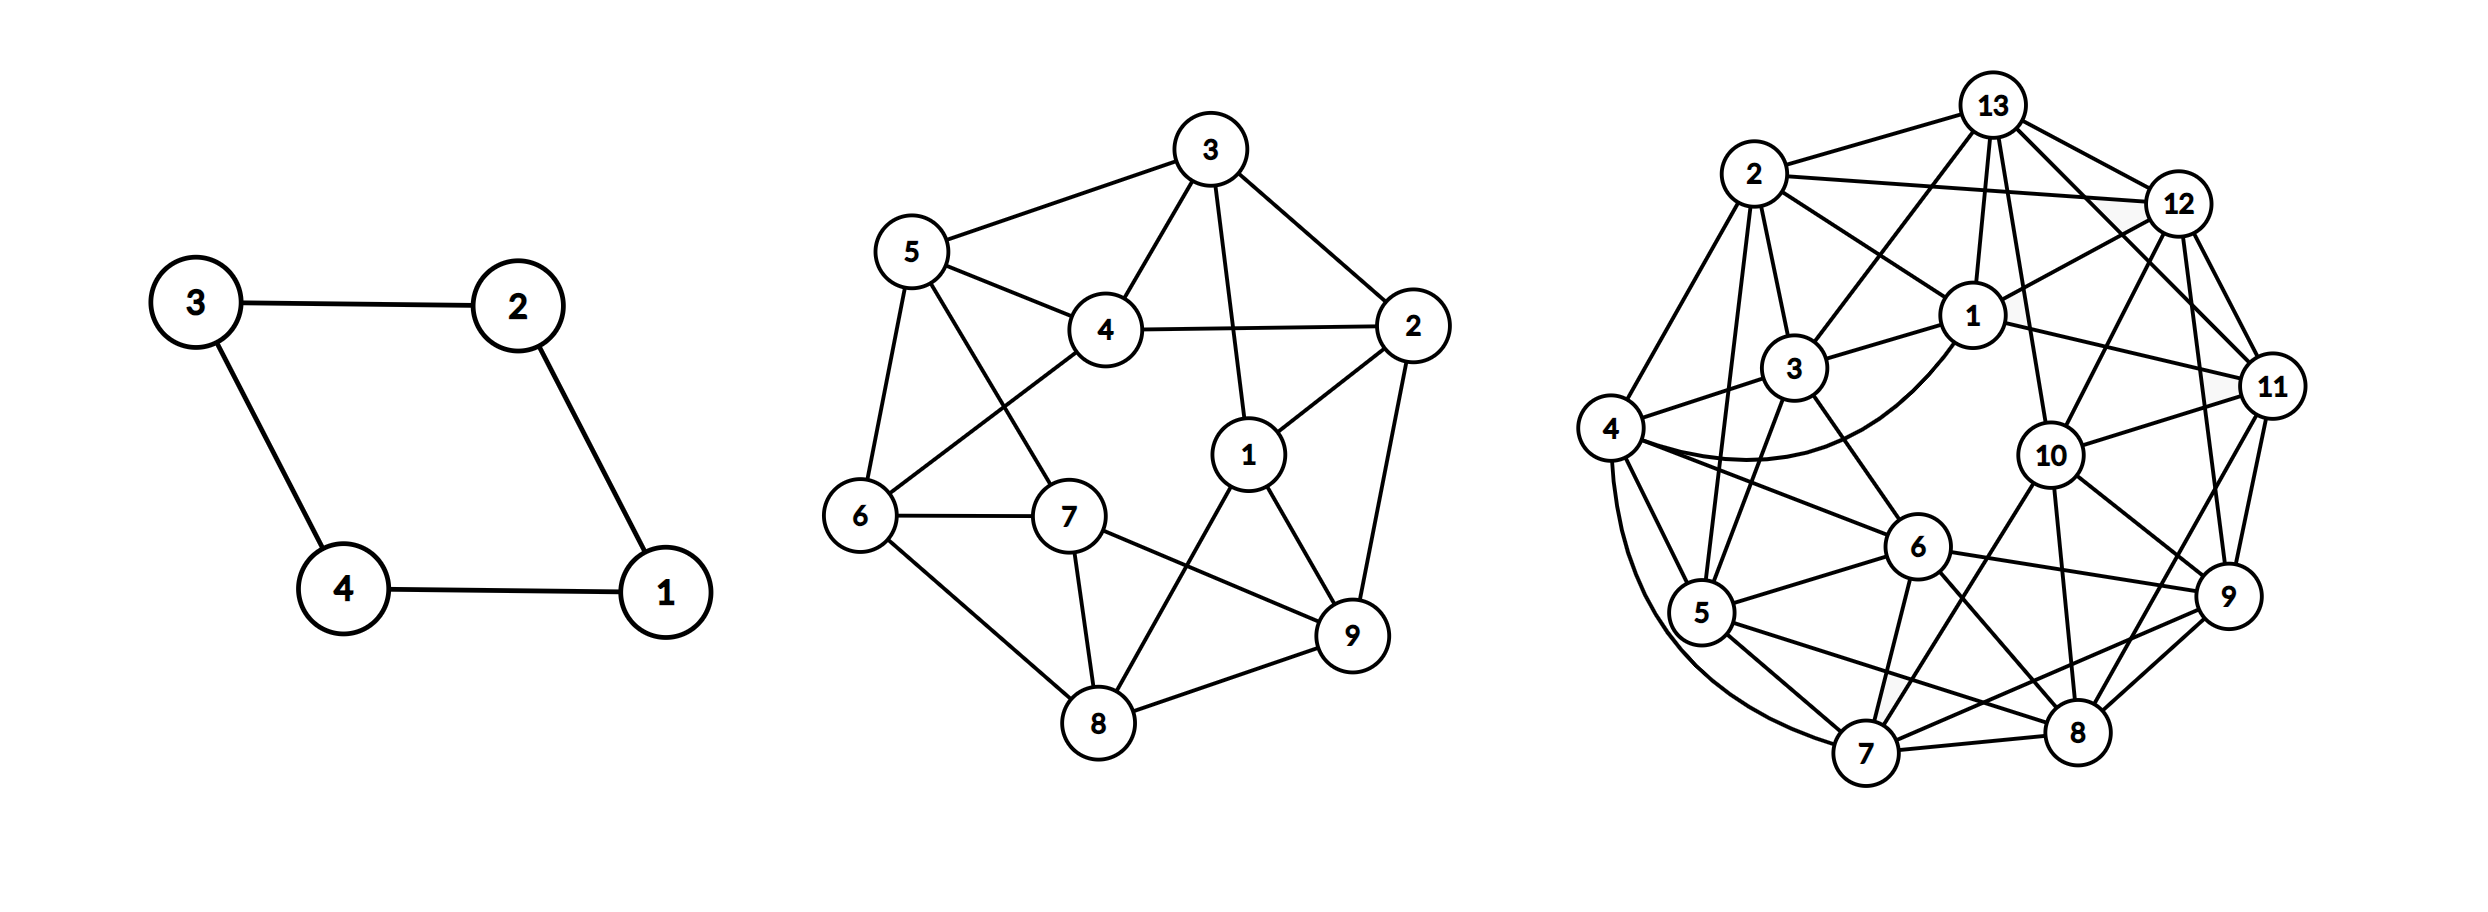
\includegraphics[width=12cm]{n2n4}
\end{center}

Graf vyvracející tuto větu lze sestrojit pro libovolné sudé $n$ například následujícím algoritmem (pouze intuitivně bez důkazu korektnosti):

$2n + 1$ návštěvníků se postaví do kruhu a každý udělí ránu $\frac{n}{2}$ kolegům, které má bezprostředně napravo, a $\frac{n}{2}$ kolegům, které má nalevo. Vzdálenost dvou návštěvníků je symetrická (např. z pohledu kolegy, který je $x \le \frac{n}{2}$ kroků napravo, jsem já stejný počet $x$ kroků nalevo). V takové rvačce jsou všechny rány vzájemné.
\qed

\newpage
\section*{Zadání 3}

Ukažte, že bipartitní graf neobsahuje lichou kružnici.

\subsection*{Řešení}

Uvažujme bipartitní graf. Definujme cyklosled jako sled v tomto grafu, ve kterém se neopakují vrcholy s výjimkou prvního a posledního vrcholu, které jsou stejné.
Každá kružnice lze jednoznačně určit nějakým cyklosledem. Každý bipartitní cyklosled má nutně sudý počet hran, aby skončil v té samé partitě -- hrany vedou pouze mezi partitami.
Protože neexistuje cyklosled liché délky, nemůže existovat ani lichá kružnice -- bylo by ji možné popsat lichým cyklosledem (spor).
\qed

\end{document}